\chapter{\IfLanguageName{dutch}{Proof of concept}{Proof of concept}}%
\label{ch:proof-of-concept}

\section{Proof of Concept: Real-time Monitoring via Centrale en Edge Databases}

Deze proof of concept heeft als doel het prestatieverschil te analyseren tussen twee implementaties voor real-time monitoring: een traditionele centrale database-architectuur (Gebouw A) en een edge computing-architectuur met lokale verwerking (Gebouw B). De focus ligt op typische IoT-sensordata zoals \ce{CO2}-metingen, temperatuur en luchtdruk.

Beide scenario's worden opgezet met Docker Compose om gescheiden en reproduceerbare testomgevingen te garanderen. Binnen elk scenario worden verschillende databases getest met meerdere datapartitioneringstechnieken (zoals range-based en list-based partitionering) om te bepalen welke het meest geschikt is voor centrale versus gedistribueerde verwerking.
\section{Functionele en niet-functionele Eisen}

\subsection{Functionele eisen}

De functionele eisen beschrijven wat het systeem concreet moet doen. Voor deze proof of concept binnen de HoGent-use case werden volgende functionele eisen gedefinieerd:

\begin{itemize}
    \item Het systeem moet om de 5 seconden de waarden van \ce{CO2}, temperatuur en luchtdruk registreren.
    \item Het systeem moet een waarschuwing tonen wanneer de \ce{CO2}-waarde de drempel van 800 ppm overschrijdt.
    \item Het systeem moet real-time grafieken tonen met de evolutie van de \ce{CO2}-waarden.
    \item Het systeem moet historische meetgegevens kunnen opvragen per lokaal.
    \item Het systeem moet logs bijhouden van wanneer drempelwaarden zijn overschreden.
    \item Het systeem moet foutmeldingen tonen bij verbindingsproblemen met de database of edge-node.
\end{itemize}

\subsection{Niet-functionele eisen}

Niet-functionele eisen beschrijven de kwaliteitseigenschappen van het systeem. Dit zijn de niet-functionele eisen voor het systeem:

\begin{itemize}
    \item \textbf{Performantie (Must):} Het systeem moet lage latentie hebben ($<$ 500 ms) bij het tonen van nieuwe meetdata.
    \item \textbf{Schaalbaarheid (Must):} Het systeem moet uitbreidbaar zijn naar meerdere lokalen zonder herconfiguratie. Ook horizontale schaalbaarheid over meerdere nodes moet ondersteund worden zonder prestatiedaling.
    \item \textbf{Fouttolerantie (Must):} Het systeem moet blijven functioneren bij netwerkstoringen of node-uitval, zonder dataverlies.
    \item \textbf{Offline werking en synchronisatie (Should):} Het systeem moet tijdelijk lokaal data kunnen opslaan en veilig synchroniseren zodra netwerkverbinding is hersteld.
    \item \textbf{Lokale verwerking (Must):} De edge-node moet in staat zijn om data lokaal te verwerken om latentie en netwerkbelasting te minimaliseren.
    \item \textbf{Geheugengebruik en CPU-belasting (Should):} De database moet efficiënt werken op edge-devices met beperkte hardwarecapaciteit.
    \item \textbf{Doorvoersnelheid (Must):} Het systeem moet hoge frequenties van sensordata kunnen verwerken (inserts per seconde).
    \item \textbf{Gegevensconsistentie (Must):} Alle nodes moeten beschikken over een betrouwbare en gelijke data.
    \item \textbf{Beheer en onderhoud (Should):} De configuratie, monitoring en foutafhandeling van het systeem moeten eenvoudig zijn.
    \item \textbf{Beveiliging (Must):} Data moet veilig worden opgeslagen en enkel toegankelijk zijn voor bevoegde gebruikers.
    \item \textbf{Automatische compressie en retentie (Could):} Het systeem moet automatisch oudere gegevens kunnen comprimeren of verwijderen. Zo blijft de opslag beperkt en raakt de edge-node niet vol. Bijvoorbeeld: alleen de data van de laatste 7 dagen wordt volledig bewaard, oudere data wordt samengevat of verwijderd.
\end{itemize}

\section{Architectuur van de testopstelling}
\label{sec:architectuur-testopstelling}

De testopstelling is gebaseerd op een simulatie van een school met twee gebouwen: Gebouw A en Gebouw B. Elk gebouw stelt een ander soort database-architectuur voor. Op die manier kan getest worden wat het verschil is tussen centrale opslag van data en lokale verwerking aan de rand van het netwerk (edge computing).

\subsection{Gebouw A: Centrale verwerking}

Gebouw A stelt een centrale serverruimte voor waar alle meetgegevens verzameld worden. De data van de sensoren wordt naar deze centrale locatie gestuurd. Daar worden de gegevens opgeslagen en verwerkt met behulp van de databases MongoDB, Cassandra of TimescaleDB. Alles gebeurt dus op een centrale plaats, zonder verdeling over meerdere locaties.

\subsection{Gebouw B: Edge-verwerking per lokaal}

Gebouw B stelt een edge-omgeving voor. In dit gebouw heeft elk lokaal zijn eigen edge-node, dus zijn eigen kleine database. In totaal zijn er zes lokalen (B101 tot B106). Elk lokaal gebruikt een andere combinatie van database en partitionering:

\begin{itemize}
  \item B101: MongoDB met list-partitionering
  \item B102: MongoDB met range-partitionering
  \item B103: Cassandra met list-partitionering
  \item B104: Cassandra met range-partitionering
  \item B105: TimescaleDB met list-achtige partitionering
  \item B106: TimescaleDB met range-partitionering
\end{itemize}

De sensordata wordt lokaal opgeslagen en verwerkt. Als bijvoorbeeld het \ce{CO2}-niveau te hoog is, wordt dit direct opgemerkt door de lokale database, zonder dat de centrale server daarvoor nodig is. De edge-databases communiceren niet met elkaar en ook niet met Gebouw A. Zo kunnen de prestaties van elk systeem apart worden gemeten.

\subsection{Verschil in resources tussen centrale en edge-opstelling}

Om het verschil tussen een centrale en een edge-architectuur realistisch te simuleren, werden in Docker Compose verschillende CPU en geheugenlimieten ingesteld.
 De centrale node (Gebouw A) krijgt meer resources, terwijl de edge-nodes (Gebouw B) beperkter geconfigureerd zijn.
Op die manier wordt het verschil gesimuleerd tussen een datacenteromgeving en een edge-device zoals een Raspberry Pi of IoT-controller.
 Dit benadert de typische situatie waarbij centrale systemen op krachtige infrastructuur draaien en edge-devices gebruikmaken van beperkte hardware.
\begin{table}[H]
\centering
\begin{resizebox}{\textwidth}{!}{
  \begin{tabular}{|l|c|c|}
  \hline
  \textbf{Eigenschap} & \textbf{Centrale databases (Gebouw A)} & \textbf{Edge-databases (Gebouw B)} \\
  \hline
  Geheugen (RAM) & 1024MB (1 GB) & 512MB of 768MB \\
  CPU-limiet & 1.0 core & 1.0 core \\
  Verbinding & Permanent (stabiel netwerk) & Mogelijk onstabiel of tijdelijk offline \\
  Voorbeelden van containers & \texttt{timescaledb-central}, \texttt{mongodb-central} & \texttt{mongos2}, \texttt{cassandra-edge-range}, \texttt{timescaledb-edge-list} \\
  \hline
  \end{tabular}
}
\end{resizebox}
\caption{Simulatie van resourceverschillen tussen centrale en edge-opstellingen.}
\label{tab:resources}
\end{table}

\subsection{Visueel overzicht van de architectuur}

De onderstaande figuur toont hoe de opstelling eruitziet. Links staat Gebouw A met de drie centrale databases. Rechts staan de zes lokalen van Gebouw B, elk met hun eigen edge-database. Er is geen verbinding tussen de gebouwen tijdens de tests, zodat de resultaten per systeem goed vergeleken kunnen worden.

\begin{figure}[H]
  \centering
  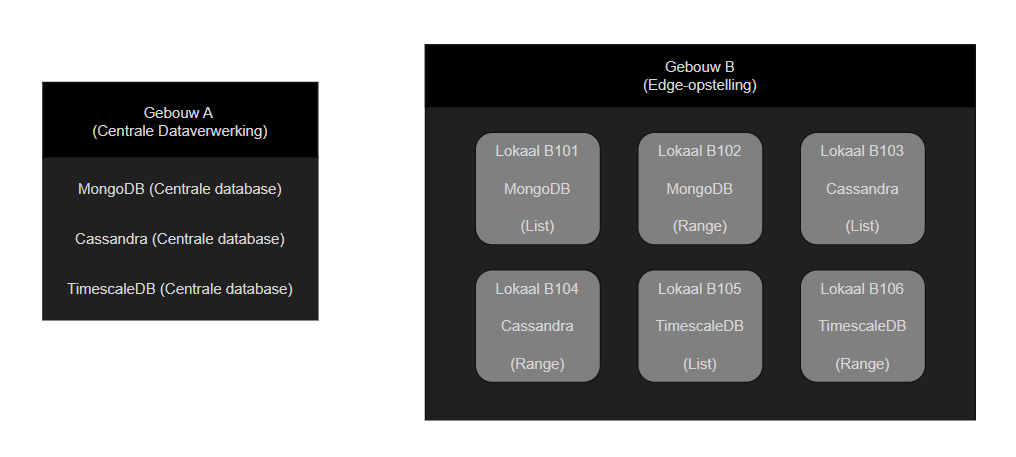
\includegraphics[width=\textwidth]{SchemaPoC.png}
  \caption{Overzicht van de testopstelling. Elke ruimte in Gebouw B heeft een eigen edge-database. In Gebouw A worden de centrale databases getest.}
  \label{fig:school-architectuur}
\end{figure}

\subsection{Testdoelen in beide gebouwen:}
\begin{itemize}
    \item Verzamelen en opslaan van meetgegevens vanuit meerdere lokalen.
    \item Detectie van drempelwaarden (\ce{CO2} > 800 ppm) en genereren van waarschuwingen.
    \item Logging van drempeloverschrijdingen en opvraging van historische data.
    \item Evaluatie van systeemprestaties bij verhoogde belasting.
    \item Analyse van schaalbaarheid en gedrag bij uitbreiding naar meerdere lokalen.
    \item Meting van latency en doorvoersnelheid.
    \item Fouttolerantie en gedrag bij netwerkstoringen of node-uitval.
    \item Monitoring van resourcegebruik (CPU, geheugen).
\end{itemize}

\section{Ontwikkeling van de Applicatie}

De proof of concept is gerealiseerd met Docker Compose en gesimuleerde sensordata. De werking van de applicatie wordt getest aan de hand van concrete functionele eisen zoals het genereren van een waarschuwing wanneer het \ce{CO2}-gehalte hoger is dan 800 ppm.
Cassandra werd in deze proof of concept via Docker gebruikt op een virtuele edge-server per lokaal. Hoewel dit geen echte IoT-hardware is, vormt het een goede benadering om de prestaties en partitionering van Cassandra in een edge-omgeving te testen.

\subsection{Architectuur}

De applicatie is opgebouwd als een real-time monitoringdashboard in een edge-omgeving met volgende componenten:

\begin{itemize}
    \item \textbf{IoT-sensor (gesimuleerd):} Genereert elke 5 seconden meetgegevens.
    \item \textbf{Edge-node:} Verwerkt en slaat lokaal data op met een te testen database-engine.
    \item \textbf{Backend (ASP.NET Core):} Verwerkt sensordata, detecteert overschrijding van drempelwaarden en verstuurt meldingen.
    \item \textbf{Frontend (React):} Visualiseert live-data en historische grafieken.
    \item \textbf{Docker Compose:} Beheert de opstelling van verschillende databases, backend en frontend in afzonderlijke containers.
\end{itemize}

\subsection{Melding bij \ce{CO2}-overschrijding}

Bij overschrijding van 800 ppm \ce{CO2}:
\begin{itemize}
    \item Wordt een rode waarschuwing getoond op het dashboard.
    \item Wordt een log-item toegevoegd aan de database.
    %\item (Optioneel) Wordt een melding verstuurd via e-mail of webhook.
\end{itemize}

\section{Tabellen en Datastructuren}

De gebruikte tabel heet \texttt{sensor\_data} en heeft een consistente structuur in alle databases.

\paragraph{Velden in \texttt{sensor\_data}:}
\begin{itemize}
    \item \texttt{sensor\_id (UUID)} - Unieke identificatie per sensor.
    \item \texttt{timestamp (TIMESTAMP)} - Tijdstip van de meting.
    \item \texttt{temperature (DOUBLE)} - Temperatuurwaarde.
    \item \texttt{co2 (INTEGER)} - CO₂-waarde in ppm.
    \item \texttt{pressure (DOUBLE)} - Luchtdruk in hPa.
    \item \texttt{status (TEXT)} - Sensorstatus ('actief', 'offline').
\end{itemize}

\paragraph{Toepassing per architectuur:}
\begin{itemize}
    \item \textbf{Gebouw A (centraal):} verschillende databases worden getest als centrale opslagoptie voor data uit alle lokalen.

    \item \textbf{Gebouw B (edge):} elk lokaal heeft een eigen edge-node waarop verschillende edge-geschikte databases worden getest.
\end{itemize}

\subsection{Uitgevoerde queries per database}
Tijdens de tests werden de sensordata telkens via een specifieke query ingevoegd in de databanken. 
De queries verschillen per database-engine en partitioneringsstrategie. Hieronder worden de belangrijkste voorbeelden weergegeven.

\paragraph{Cassandra (centraal):}
\begin{verbatim}
INSERT INTO sensor_data (id, timestamp, temperature, co2, pressure, building, room)
VALUES (?, ?, ?, ?, ?, ?, ?)
\end{verbatim}
Deze query werd via een prepared statement uitgevoerd met de Node.js-driver. 
Bij de edge-configuraties werd de kolomvolgorde aangepast afhankelijk van de gekozen partitionering (list- of range-based).

\paragraph{MongoDB (centraal):}
\begin{verbatim}
db.collection("sensor_data").insertOne(sensorData)
\end{verbatim}
Voor de consistentietests werd gebruikgemaakt van een majority-write concern:
\begin{verbatim}
db.collection("sensor_data").insertOne(sensorData, { writeConcern: { w: "majority" } })
\end{verbatim}

\paragraph{TimescaleDB (centraal):}
\begin{verbatim}
INSERT INTO sensor_data (id, timestamp, temperature, co2, pressure, building, room)
VALUES ($1, $2, $3, $4, $5, $6, $7)
\end{verbatim}
De parameters worden ingevuld met gegenereerde sensordata via de functie generateSensorData.


\section{Workload Simulatie}

\paragraph{Datageneratie met Faker.js}
De sensordata worden gegenereerd met behulp van \texttt{Faker.js}. Voor elke meting worden 
een tijdstip, temperatuur, \ce{CO2}-waarde en luchtdruk vastgelegd. Er wordt bovendien 
een kans van 5\% toegevoegd dat er een afwijkende \ce{CO2}-waarde (\textgreater 800 ppm) optreedt, 
zodat anomalieën in de data realistisch gesimuleerd worden.

\begin{verbatim}
function generateRandomData(building, index = 0, prevData = null, fixedRoom = null) {
  const timestamp = new Date(START_TIME.getTime() + index * 5000);
  const room = fixedRoom ?? getRandomRoom(building);

  function varyValue(prev, min, max, maxDelta) {
    if (prev === null) {
      return faker.number.float({ min, max, multipleOf: 0.1 });
    }
    let next = prev + faker.number.float({ min: -maxDelta, max: maxDelta, multipleOf: 0.1 });
    return Math.min(max, Math.max(min, Number(next.toFixed(1))));
  }

  let co2;
  const shouldTriggerWarning = Math.random() < 0.05;
  if (shouldTriggerWarning) {
    co2 = varyValue(prevData ? prevData.co2 : null, 801, 850, 20);
  } else {
    co2 = varyValue(prevData ? prevData.co2 : null, 350, 800, 20);
  }

  return {
    _id: faker.string.uuid(),
    timestamp,
    temperature: varyValue(prevData?.temperature, 18, 28, 0.2),
    co2: Math.round(co2),
    pressure: varyValue(prevData?.pressure, 990, 1030, 0.3),
    building,
    room,
  };
}
\end{verbatim}


\paragraph{Data-invoer}
Via Node.js-scripts wordt data naar de databases geschreven. Elke container ontvangt data alsof die afkomstig is uit een lokaal.

Elke test wordt herhaald voor verschillende database-engines in zowel Gebouw A als Gebouw B. Zo kan geëvalueerd worden welke database het best presteert binnen het gekozen architecturale model.

\paragraph{Functionele tests}
In beide gebouwen worden dezelfde functionele eisen getest:
\begin{itemize}
    \item Waarschuwing tonen als \ce{CO2} > 800 ppm.
    \item Sensorstatus tonen op dashboard.
    \item Logging van overschrijdingen.
    \item Tijdige en correcte opslag van data.
\end{itemize}

\paragraph{Niet-functionele tests}
De volgende prestatiekenmerken worden geëvalueerd:
\begin{itemize}
    \item \textbf{Doorvoersnelheid:} hoeveel metingen kunnen per seconde worden verwerkt?
    \item \textbf{Latency:} hoe snel worden data en waarschuwingen zichtbaar?
    \item \textbf{Verticale schaalbaarheid:} hoe reageert een database op meerdere gelijktijdige bewerkingen binnen één edge-node?
    \item \textbf{Fouttolerantie:} wat gebeurt er bij netwerk- of node-uitval?
    \item \textbf{Offline gedrag:} blijft Gebouw B operationeel zonder internet?
\end{itemize}

\section{Visualisatie van sensordata in de frontend}

Voor de realtime visualisatie van sensordata werd een webinterface gebouwd met React.
 De interface stelt gebruikers in staat om live metingen van CO$_2$, temperatuur en luchtdruk te bekijken, afkomstig van verschillende gebouwen (zoals Gebouw A en B) en ondersteund door drie databackends: MongoDB, Cassandra en TimescaleDB.

De frontend maakt gebruik van de \texttt{axios}-bibliotheek om op regelmatige tijdstippen sensorgegevens op te halen via API-endpoints van de ASP.NET Core-backend.
 Afhankelijk van de geselecteerde configuratie (gebouw en database) wordt automatisch een dynamische lijngrafiek weergegeven, gevisualiseerd met de \texttt{Recharts}-bibliotheek.

Een waarschuwing wordt getoond wanneer het \ce{CO2}-niveau een bepaalde drempelwaarde overschrijdt. Dit stelt gebruikers in staat om snel te reageren op afwijkende omstandigheden binnen het monitoring systeem.

Een voorbeeld van de gebruikte logica in React:

\begin{verbatim}
useEffect(() => {
  const interval = setInterval(async () => {
    try {
      const res = await axios.get('/api/sensordata/latest', { params: { building, type } });
      setData(prev => {
        const combined = [...prev.slice(-19), res.data];
        return combined.sort((a, b) => new Date(a.timestamp) - new Date(b.timestamp));
      });
    } catch (err) {
      console.error('Fout bij ophalen data:', err.message);
    }
  }, 5000);

  return () => clearInterval(interval);
}, [building, type]);
\end{verbatim}

Gebruikers kunnen in de interface kiezen van welk gebouw en welke database ze data willen zien. 
 Daarna verschijnt automatisch een grafiek met de meest recente meetwaarden.

\begin{figure}[H]
	\centering
	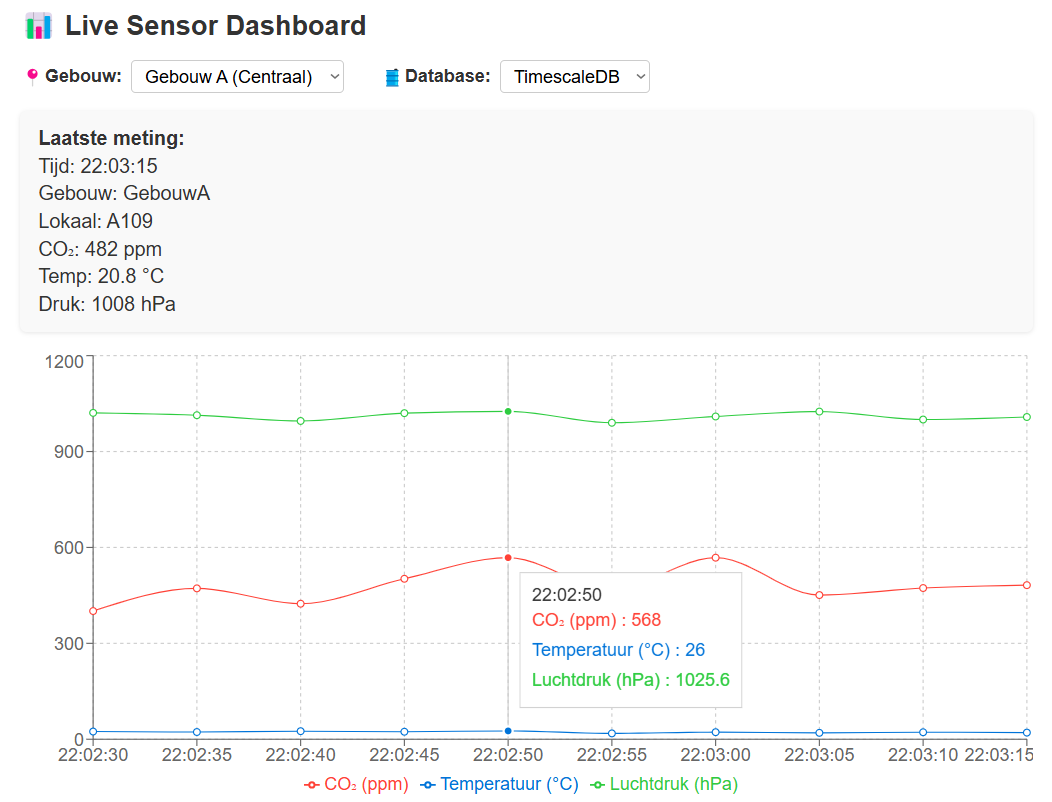
\includegraphics[width=0.8\textwidth]{GebouwA_TimeScale_Website.png}
	\caption{Frontendweergave met centrale database-architectuur (TimescaleDB, Gebouw A).}
    \label{fig:gebouw-a-architecture}
\end{figure}

\begin{figure}[H]
    \centering
    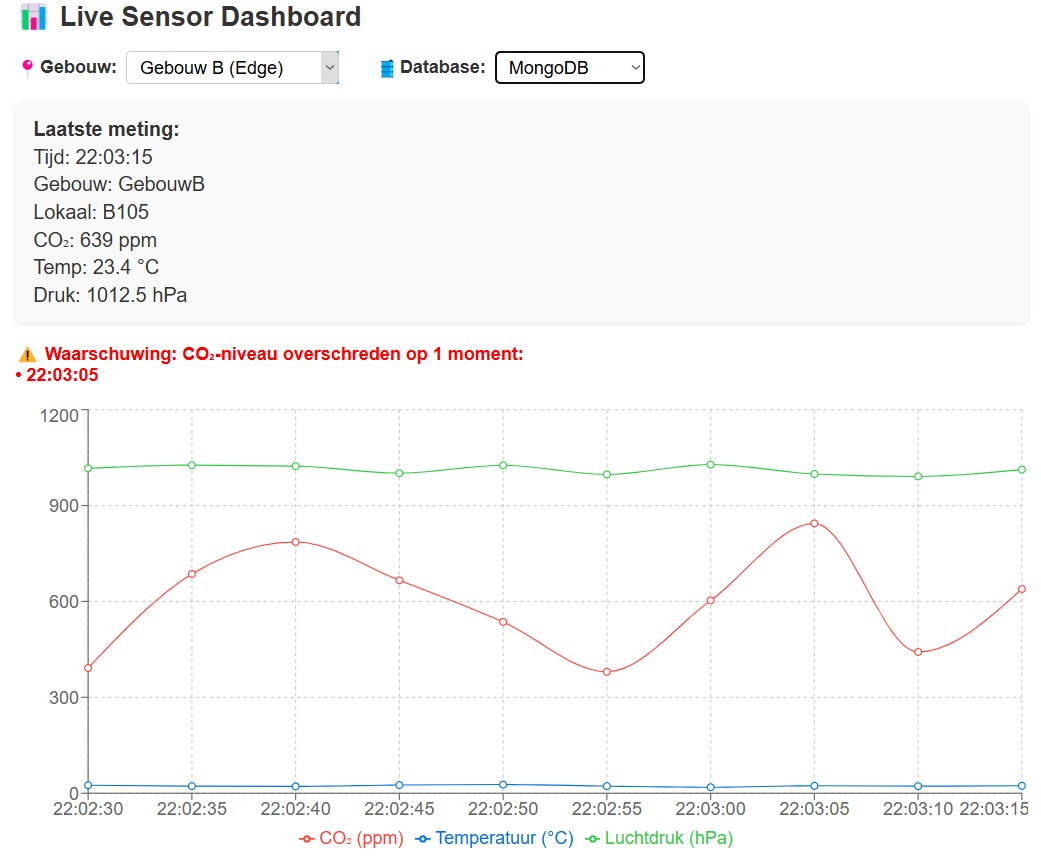
\includegraphics[width=0.8\textwidth]{GebouwB_MongoDb_Website.png}
    \caption{Frontendweergave met edge computing-architectuur (MongoDB, Gebouw B).}
    \label{fig:gebouw-b-architecture}
\end{figure}

De volledige code van het dashboard is beschikbaar via GitHub: \\
\href{https://github.com/WoutVC/sensor-dashboard/blob/master/src/components/LiveDashboard.js}{LiveDashboard.js}

\section{Resultaten en Grafieken}
Voor de prestatietests (latentie, throughput, schaalbaarheid en consistentie) behalve de fouttolerantietest werden telkens vijf runs uitgevoerd en het gemiddelde berekend om een representatief resultaat te verkrijgen.

De resultaten van deze tests, uitgevoerd met het script \href{https://github.com/WoutVC/bachelorproef2024/blob/main/proof_of_concept/backend/POCTests.js}{POCTests.js},
 zijn hieronder weergegeven in grafieken. Ze tonen hoe de verschillende databases presteren op vlak van snelheid, betrouwbaarheid en schaalbaarheid in een edge-omgeving.
\subsection{Latency}

\begin{figure}[H]
	\centering
	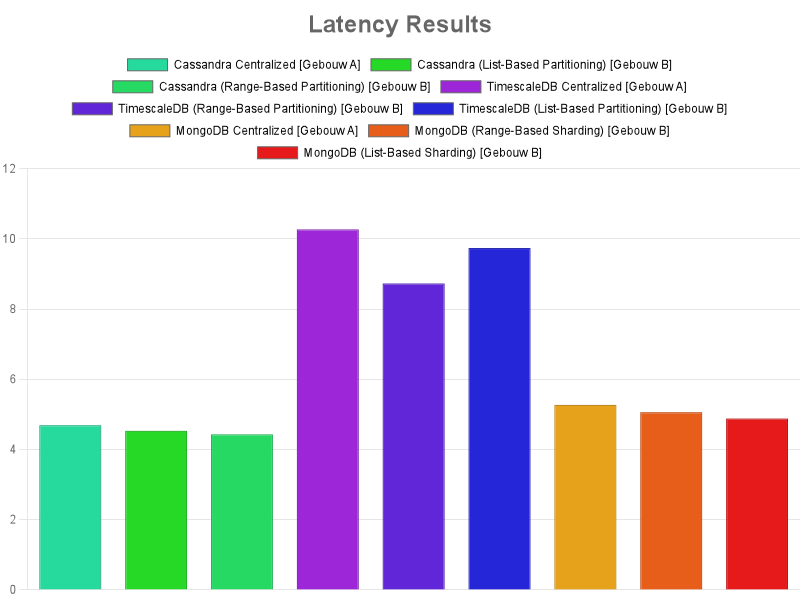
\includegraphics[width=0.8\textwidth]{charts/Latency.png}
	\caption{Latentie van Cassandra, MongoDB en TimescaleDB (tijd om 1 record op te slaan).}
	\label{fig:latency-comparison}
\end{figure}

\paragraph{Hoe werd latentie getest?}
Voor deze test werd de functie \texttt{testRealtimeLatency()} gebruikt uit het script. Elke seconde werd een meetwaarde naar de database gestuurd. Daarna werd gemeten hoeveel milliseconden het duurde om die actie uit te voeren. Dit werd meerdere keren herhaald om een gemiddelde te berekenen.

\begin{verbatim}
async function testRealtimeLatency(client, queryFn, label, intervalMs = 1000, durationSeconds = 10) {
  const records = Math.floor(durationSeconds * 1000 / intervalMs);
  let totalLatency = 0;
  for (let i = 0; i < records; i++) {
    const start = performance.now();
    await executeQuery(queryFn);
    const end = performance.now();
    totalLatency += (end - start);
    await sleep(intervalMs);
  }
  return totalLatency / records;
}
\end{verbatim}

\paragraph{Resultaat en analyse:}
De laagste latentie werd gemeten bij \textit{Cassandra (Range-Based Partitioning)} met 4.43 ms, gevolgd door \textit{Cassandra (List-Based Partitioning)} (4.53 ms) en \textit{MongoDB (List Partitioning)} (4.88 ms). De traagste database was \textit{TimescaleDB centraal} (10.27 ms). Dit toont aan dat vooral Cassandra en MongoDB sneller reageren in een realtime edge-context.

\subsection{Throughput}

\begin{figure}[H]
	\centering
	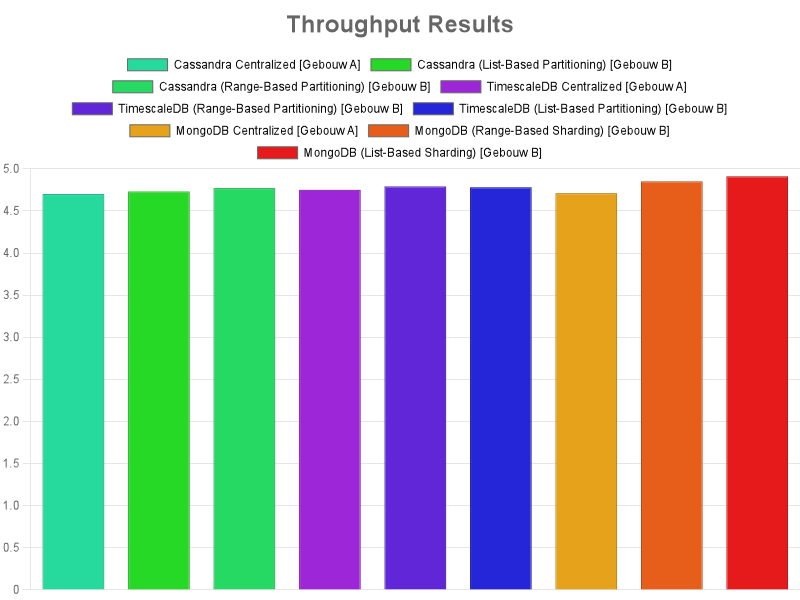
\includegraphics[width=0.8\textwidth]{charts/Throughput.png}
	\caption{Throughput: hoeveel meetwaarden per seconde werden opgeslagen.}
	\label{fig:throughput-comparison}
\end{figure}

\paragraph{Hoe werd throughput getest?}
De functie \texttt{testRealtimeThroughput()} werd hiervoor gebruikt. Tijdens deze test werd gedurende tien seconden om de 200 milliseconden een datapunt ingestuurd. Daarna werd berekend hoeveel meetpunten per seconde de database kon verwerken.

\begin{verbatim}
async function testRealtimeThroughput(queryFn, label, intervalMs = 200, durationSeconds = 10) {
  let operationCount = 0;
  const start = performance.now();
  const endTime = start + durationSeconds * 1000;
  while (performance.now() < endTime) {
    await executeQuery(queryFn, label);
    operationCount++;
    await sleep(intervalMs);
  }
  const elapsedSeconds = (performance.now() - start) / 1000;
  return operationCount / elapsedSeconds;
}
\end{verbatim}

\paragraph{Resultaat en analyse:}
\textit{MongoDB (List Partitioning)} behaalde de beste score met 4.91 records/s. De andere databases zaten dicht bij elkaar (tussen 4.7 en 4.8 records/s). Dit suggereert dat alle systemen vlot genoeg zijn om continue datastromen te verwerken.

\subsection{Scalability}

\begin{figure}[H]
	\centering
	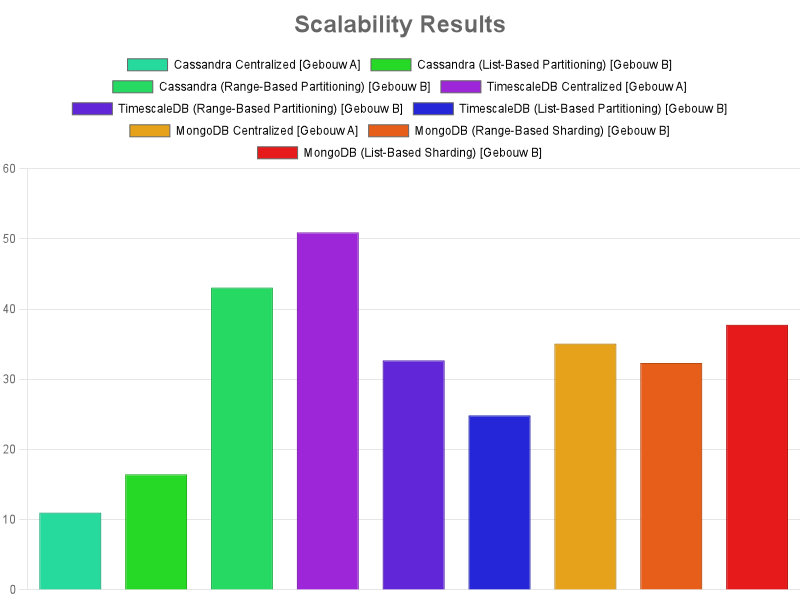
\includegraphics[width=0.8\textwidth]{charts/Scalability.png}
	\caption{Verticale schaalbaarheid: tijdsduur bij gelijktijdige bewerkingen binnen één database-instantie.}
	\label{fig:scalability-comparison}
\end{figure}

\paragraph{Hoe werd schaalbaarheid getest?}
De functie \texttt{testScalability()} simuleerde hoeveel tijd het kost om meerdere meetwaarden tegelijk op te slaan (bijvoorbeeld 10, 50 of 100 gelijktijdige inserts). Deze test evalueert de \textbf{verticale schaalbaarheid} van een database: hoe goed één node of container omgaat met piekbelasting door meerdere gelijktijdige schrijfacties.

\begin{verbatim}
async function testScalability(queryFn, label, scaleFactors) {
  let durations = [];
  for (const factor of scaleFactors) {
    const concurrentOps = Array.from({ length: factor }, () => executeQuery(queryFn));
    const start = performance.now();
    await Promise.all(concurrentOps);
    const end = performance.now();
    durations.push({ factor, duration: end - start });
  }
  return durations.reduce((a, b) => a + b.duration, 0) / durations.length;
}
\end{verbatim}

\paragraph{Resultaat en analyse:}
\textit{TimescaleDB centraal} presteerde het best met 50.93 (laagste verwerkingstijd bij hoge load), gevolgd door \textit{Cassandra (Range Partitioning)} (43.06). De zwakste resultaten kwamen van \textit{Cassandra (List Partitioning)} (16.45). Dit toont dat TimescaleDB zeer goed schaalt op één node.

\subsection{Consistentie}

\begin{figure}[H]
\centering
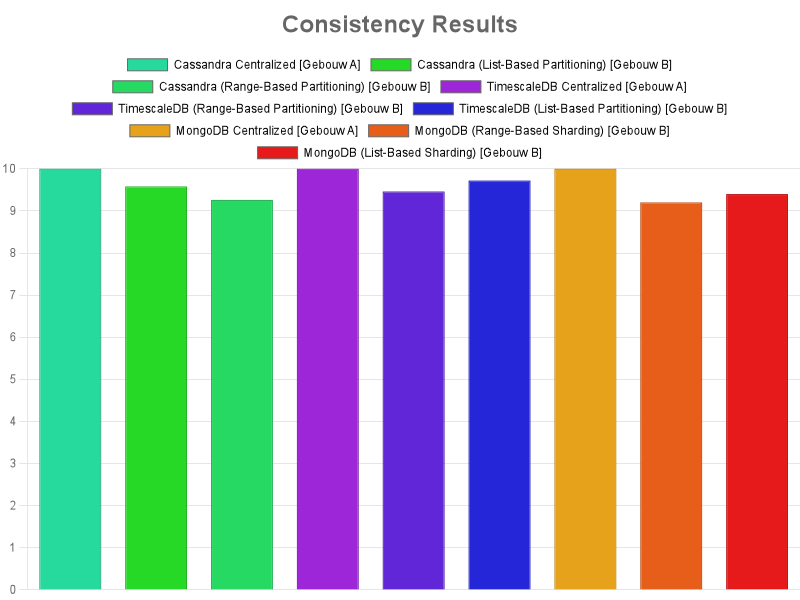
\includegraphics[width=0.8\textwidth]{charts/Consistency.png}
\caption{Consistentie: hoeveel records onmiddellijk beschikbaar waren.}
\label{fig:consistency-comparison}
\end{figure}

\paragraph{Hoe werd consistentie getest?}
De functie \texttt{testConsistency()} schreef 100 records weg. Daarna werd bij intervallen van 0, 500, 1000, 2000 en 3000 ms gecontroleerd hoeveel records zichtbaar waren.  
Voor edge-databases werd kunstmatig replica-lag gesimuleerd door 5-15\% van de records tijdelijk niet zichtbaar te maken.

\begin{verbatim}
async function testConsistency(client, queryFn, label) {
  const baseTimestamp = new Date();
  const timestamps = [...Array(10)].map((_, i) => new Date(baseTimestamp.getTime() + i * 1000));
  await Promise.all(timestamps.map(ts => queryFn(ts)));
  const waitIntervals = [0, 500, 1000, 2000];
  for (const delay of waitIntervals) {
    await sleep(delay);
    // tel aantal zichtbare records op basis van timestamp
  }
}
\end{verbatim}

\paragraph{Resultaat en analyse:}
\textit{Cassandra Centralized} en \textit{MongoDB Centralized} scoorden het maximum (10/10). Edge-configuraties haalden iets lagere waarden: bv. \textit{Cassandra (List)} 9.58 en \textit{MongoDB (Range)} 9.20. Dit weerspiegelt de verwachte replica-lag in een edge-omgeving.

\subsection{Fouttolerantie}

\begin{figure}[H]
    \centering
    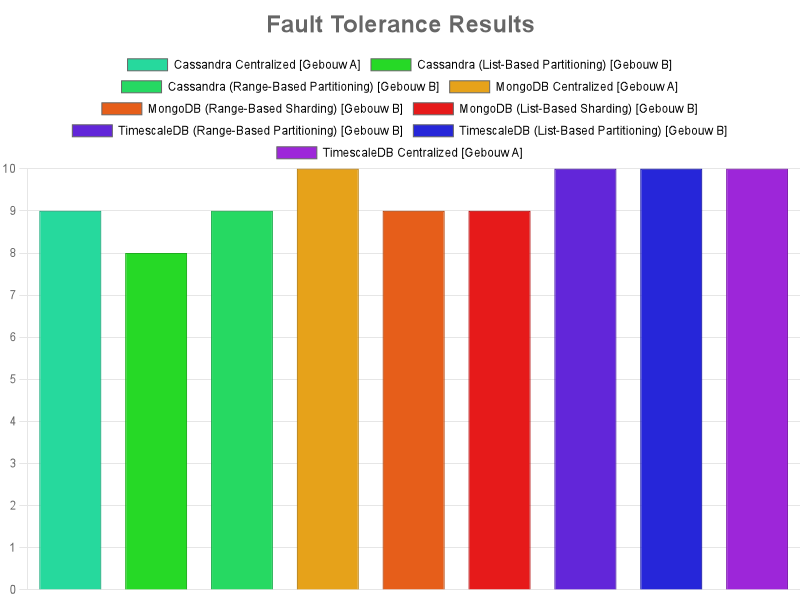
\includegraphics[width=0.8\textwidth]{charts/Fault_Tolerance.png}
    \caption{Fouttolerantie: werking na onderbreking van de verbinding.}
    \label{fig:fault-tolerance-comparison}
\end{figure}

\paragraph{Hoe werd fouttolerantie getest?}
Tijdens deze test werd de verbinding bewust verbroken (via \texttt{shutdown()} of \texttt{close()}). Daarna werd een nieuwe client aangemaakt en opnieuw verbonden. De duur van dit herstel werd omgezet naar een score via \texttt{mapDurationToScore()}.

\begin{verbatim}
async function testFaultTolerance(client, label, createNewClient) {
  await client.shutdown();
  client = createNewClient();
  await client.connect();
  testResults.push({ metric: "Fault Tolerance", label, value: "Success" });
}

function mapDurationToScore(durationMs) {
  if (durationMs < 100) return 10;
  if (durationMs < 200) return 9;
  if (durationMs < 300) return 8;
  ...
  return 1;
}
\end{verbatim}

\paragraph{Resultaat en analyse:}
Alle databases konden opnieuw verbinding maken. \textit{TimescaleDB centraal} scoorde het hoogst (10), terwijl sommige edge-configuraties zoals \textit{Cassandra (List)} iets lager scoorden (8).

\subsection{Testresultaten en Tabeloverzicht}
Naast de grafieken biedt deze tabel een samenvatting van de testresultaten.

\begin{table}[h]
    \centering
    \resizebox{\textwidth}{!}{
    \begin{tabular}{|l|c|c|c|c|c|}
        \hline
        \textbf{Database}                                 & \textbf{Fault Tolerance} & \textbf{Scalability} & \textbf{Realtime Latency} & \textbf{Realtime Throughput} & \textbf{Consistency} \\ \hline
        Cassandra Centralized [Gebouw A]                  & 9                        & 10.98                & 4.69                      & 4.70                         & 10                   \\ \hline
        Cassandra (List-Based Partitioning) [Gebouw B]    & 8                        & 16.45                & 4.53                      & 4.73                         & 9.58                 \\ \hline
        Cassandra (Range-Based Partitioning) [Gebouw B]   & 9                        & 43.06                & 4.43                      & 4.77                         & 9.26                 \\ \hline
        TimescaleDB Centralized [Gebouw A]                & 10                       & 50.93                & 10.27                     & 4.75                         & 10                   \\ \hline
        TimescaleDB (Range-Based Partitioning) [Gebouw B] & 10                       & 32.68                & 8.73                      & 4.79                         & 9.46                 \\ \hline
        TimescaleDB (List-Based Partitioning) [Gebouw B]  & 10                       & 24.85                & 9.74                      & 4.78                         & 9.72                 \\ \hline
        MongoDB Centralized [Gebouw A]                    & 10                       & 35.07                & 5.27                      & 4.71                         & 10                   \\ \hline
        MongoDB (Range-Based Sharding) [Gebouw B]         & 9                        & 32.32                & 5.06                      & 4.85                         & 9.20                 \\ \hline
        MongoDB (List-Based Sharding) [Gebouw B]          & 9                        & 37.76                & 4.88                      & 4.91                         & 9.40                 \\ \hline
    \end{tabular}
    }
    \caption{Vergelijking van prestaties tussen Cassandra, MongoDB en TimescaleDB in centrale (Gebouw A) en edge (Gebouw B) configuraties.}
    \label{tab:test-results}
\end{table}

\subsection{Conclusie}
De evaluatie van de databases is gebaseerd op een gewogen scoresysteem (\href{https://github.com/WoutVC/bachelorproef2024/blob/main/proof_of_concept/backend/analyzeResults.js}{analyzeResults.js}), waarbij de volgende stappen worden uitgevoerd:

\paragraph{Consolidatie van resultaten:} 
Voor elke database worden de resultaten per meetwaarde samengevoegd. Voor meetwaarden zoals schaalbaarheid (Scalability), waarvoor meerdere metingen beschikbaar zijn, wordt het gemiddelde berekend.

\paragraph{Normalisatie van scores:} 
De numerieke scores voor elke meetwaarde worden genormaliseerd naar een schaal van 0 tot 1 op basis van het minimum en maximum onder alle databases:
\[
\text{Genormaliseerde score} = \frac{\text{Waarde} - \text{Minimum}}{\text{Maximum} - \text{Minimum}}
\]
Indien minimum en maximum gelijk zijn, wordt een neutrale score toegekend (bijvoorbeeld 0.5).

Voor meetwaarden waarbij een hogere score beter is (zoals throughput, schaalbaarheid, fouttolerantie en consistentie) wordt deze genormaliseerde score direct gebruikt. Voor meetwaarden waarbij een lagere score beter is (zoals latentie) wordt de genormaliseerde score omgekeerd berekend, zodat een lagere oorspronkelijke waarde leidt tot een hogere genormaliseerde score.

\paragraph{Gewogen totaalscore:} 
De genormaliseerde scores worden vervolgens gewogen op basis van vooraf bepaalde belangrijkheidsfactoren per meetwaarde en opgeteld tot een totaalscore per database.


\textbf{Toepassing van gewichten:} Elke meetwaarde krijgt een gewicht op basis van het relatieve belang voor edge computing. De toegepaste gewichten zijn als volgt:
\begin{itemize} 
	\item \textbf{Fouttolerantie - 20\% (Must Have):}  
	De apparaten aan de rand van het netwerk moeten goed blijven werken, zelfs bij tijdelijke stroom- of netwerkproblemen. Gegevens mogen niet verloren gaan.

	\item \textbf{Schaalbaarheid - 20\% (Should Have):}  
	Aangezien er mogelijk honderden lokalen zijn, moet het systeem makkelijk groter gemaakt kunnen worden zonder dat het trager wordt.

	\item \textbf{Verwerkingssnelheid - 15\% (Should Have):}  
	Het systeem moet snel genoeg zijn om alle gegevens van de sensoren op tijd te verwerken.

	\item \textbf{Latentie - 15\% (Should Have):}  
	De vertraging tussen het meten van gegevens en het verwerken of opslaan ervan moet zo klein mogelijk zijn om real-time inzichten mogelijk te maken.

	\item \textbf{Gegevensconsistentie - 10\% (Could Have):}  
	Het is minder erg als data niet altijd 100 \% gelijk is op alle plaatsen, zolang het systeem maar snel en beschikbaar blijft. Toch is het belangrijk bij het samenvoegen van meetgegevens.
\end{itemize}

\paragraph{Berekening van totaalscores:} 
Om de verschillende databases goed met elkaar te kunnen vergelijken, werd voor elke database een totaalscore berekend. Deze score is gebaseerd op een combinatie van vijf belangrijke eigenschappen: fouttolerantie, schaalbaarheid, latency (vertraging), throughput (verwerkingssnelheid) en consistentie. Hoe beter een database scoorde op deze eigenschappen, hoe hoger haar totaalscore. Lagere latency werd hierbij als beter beschouwd. Alle scores zijn genormaliseerd zodat ze eerlijk met elkaar vergeleken kunnen worden.

\paragraph{Totaalscores en rangschikking:}

Op basis van deze berekening ziet de top 3 er als volgt uit:

\begin{itemize}
    \item \textbf{MongoDB Centralized [Gebouw A]} Score: \textbf{6.95}  
    Deze configuratie behaalde de hoogste totaalscore. Vooral de combinatie van consistente prestaties en fouttolerantie zorgt voor een sterke algemene score.

    \item \textbf{MongoDB (List-Based Sharding) [Gebouw B]} Score: \textbf{6.84}  
    Deze configuratie scoorde goed op throughput en fouttolerantie, waardoor ze zeer geschikt is voor real-time verwerking aan de rand van het netwerk.

    \item \textbf{TimescaleDB Centralized [Gebouw A]} Score: \textbf{6.70}  
    Deze configuratie onderscheidde zich voornamelijk door een hoge schaalbaarheid en stabiele prestaties.
\end{itemize}

\paragraph{Conclusie:}
De testresultaten tonen aan dat \textbf{MongoDB} zowel in centrale als edge-omgevingen zeer goed presteert.  
Opvallend is dat \textbf{MongoDB Centralized} het hoogst scoorde (6.95), wat deels te verklaren is doordat alle databases in een lokale Docker-omgeving draaiden zonder echte netwerkvertraging.  
Binnen de edge-omgeving is \textbf{MongoDB (List-Based Sharding)} de beste keuze (6.84), vooral dankzij zijn hoge throughput en fouttolerantie.  
\textbf{TimescaleDB} blijft interessant door zijn uitstekende schaalbaarheid, terwijl \textbf{Cassandra} zich onderscheidt met de laagste latentie.  
Welke database het meest geschikt is, hangt dus af van de specifieke vereisten: robuustheid en balans (MongoDB), schaalbaarheid (TimescaleDB) of lage latentie (Cassandra).